\documentclass{article}
\usepackage{graphicx} % Required for inserting images
% --- Math packages ---
\usepackage{amsmath}   % core math environments
\usepackage{amssymb}   % extra symbols (e.g., \mathbb)
\usepackage{amsthm}    % theorem/lemma/proposition environments
\usepackage{mathtools} % extensions to amsmath (recommended)
\usepackage{tikz}
\usetikzlibrary{arrows.meta,positioning,calc,fit,backgrounds,shapes.geometric}
\usepackage{booktabs}
\usepackage{subcaption}

% --- Unified TikZ styles for all game/causal diagrams ---
\tikzset{
  % Base styles
  diagram base/.style={
    >=Latex,
    every node/.style={font=\small},
    node distance=20mm,
  },
  % Game theory nodes
  player node/.style={circle, draw, thick, minimum size=8mm, inner sep=0pt, fill=white},
  terminal node/.style={rectangle, draw, thick, rounded corners=3pt, inner sep=4pt, fill=gray!10},
  % Causal diagram nodes
  endo node/.style={circle, draw, thick, minimum size=9mm, inner sep=0pt, fill=white},
  exo node/.style={circle, draw, dashed, thick, minimum size=8mm, inner sep=0pt, fill=gray!5},
  % --- MAID STYLES (Standard Conventions) ---
  maid decision/.style={rectangle, draw, thick, minimum size=9mm, minimum height=8mm, inner sep=2pt, fill=blue!5},
  maid utility/.style={diamond, draw, thick, aspect=1.3, minimum width=12mm, inner sep=0pt, fill=red!5},
  maid chance/.style={ellipse, draw, thick, minimum size=9mm, inner sep=1pt, fill=white},
  % Information set
  info set/.style={densely dashed, thick, gray},
  % Edge labels
  edge label/.style={font=\small, fill=white, inner sep=1pt},
}

% --- Common math fonts/notation helpers (optional but standard) ---
\usepackage{bbm}       % \mathbbm{1} indicator (optional)
\usepackage{bm}        % bold math symbols \bm{...} (optional)
\DeclareMathOperator*{\argmax}{arg\,max}
\DeclareMathOperator*{\argmin}{arg\,min}
\providecommand{\do}{\mathrm{do}}

% --- If you want clickable equation refs (optional) ---
\usepackage{hyperref}

\title{Causality and game theory: structural connections}
\author{Gabe Smithline}
\date{December 2025}

\begin{document}

\maketitle

\section{Introduction}
Causality and game theory are two mathematical frameworks for reasoning about the world, but they were built to answer different questions. Broadly, causality asks what would happen if we intervened in a system. It distinguishes association from intervention and counterfactuals, and it formalizes how outcomes change under \(\do(\cdot)\) operations and structural assumptions. Game theory asks what outcomes are stable when multiple decision-makers strategically choose actions while anticipating each other. From that, it defines solution concepts for structured strategic interactions.

At first glance, these perspectives can feel a bit at odds. Standard causal reasoning treats interventions as exogenous manipulations that sever incoming influences, whereas in a strategic setting, changing an upstream variable often changes how other agents respond. Conversely, game-theoretic reasoning is inherently counterfactual (think about the definition of a Nash equilibrium, it is reasoning about deviations), yet the relevant counterfactual in a game is rarely "hold everything else fixed" in the Pearl sense, because other agents may rationally adjust.

This tension becomes clear as soon as you ask questions that mix both lenses. What is the effect of changing the information structure? How do commitments or mechanism changes propagate through strategic responses? What is the causal contribution of introducing a new strategy into a population of strategies that will re-equilibrate? At what level can these ideas be brought together?

In this post I am going to do two things. First, I will give quick background on the objects from game theory and causality that we will actually use. Second, I will show one clean structural bridge between the two, built around Multiagent Influence Diagrams (MAIDs), and explain what it really means to ask a causal question inside a game.

\section{Background}
\subsection{Game Theory}
Game theory is a mathematical language for strategic situations: settings in which each agent’s outcome depends not only on their own decisions, but also on the decisions of others. Formally, a \emph{game} specifies (i) who the players are, (ii) what each player can do, (iii) what each player knows when they move, and (iv) how the joint choices map to payoffs. The core objects are \emph{strategies} (complete contingent plans) and \emph{solution concepts} (predictions of stable behavior under rational choice).

If you have seen game theory before, you can treat this section as a refresher. I am keeping it here because later, when we talk about interventions and equilibrium response, the details of what is a "strategy" and what is "fixed" will matter.

\paragraph{Normal-form (strategic-form) games.}
A finite normal-form game is a tuple
\[
\Gamma \;=\; \bigl(N,\,(A_i)_{i\in N},\,(u_i)_{i\in N}\bigr),
\]
where \(N=\{1,\dots,n\}\) is the set of players, \(A_i\) is player \(i\)’s (finite) action set, and \(u_i:\prod_{j\in N} A_j \to \mathbb{R}\) is player \(i\)’s payoff function. A (mixed) strategy for player \(i\) is a distribution \(\sigma_i \in \Delta(A_i)\), and a strategy profile is \(\sigma=(\sigma_1,\dots,\sigma_n)\in \prod_i \Delta(A_i)\). The expected payoff under \(\sigma\) is
\[
u_i(\sigma) = \sum_{a\in \prod_j A_j}\Bigl(\prod_{j\in N}\sigma_j(a_j)\Bigr)\,u_i(a).
\]
A game is \emph{zero-sum} (two-player) if \(u_1(a) + u_2(a) = 0\) for all \(a\) (more generally, it is \emph{constant-sum} if the sum is a constant independent of \(a\)). Otherwise, it is \emph{general-sum}. Here incentives can be partially aligned, partially opposed, and cooperation may create surplus while competition determines how it is split.

% -------------------------
% Diagram: normal-form game
% -------------------------

\begin{figure}[htbp]
\centering
\setlength{\tabcolsep}{14pt}
\renewcommand{\arraystretch}{1.4}
\begin{tabular}{@{} l cc @{}}
\toprule
 & \textbf{Cooperate (C)} & \textbf{Defect (D)} \\
\midrule
\textbf{Cooperate (C)} & $(-1,\,-1)$ & $(-7,\,-0.5)$ \\
\textbf{Defect (D)} & $(-0.5,\,-7)$ & $(-1.9,\,-1.9)$ \\
\bottomrule
\end{tabular}
\caption{A normal-form game as a payoff matrix. Rows are Player 1's actions, columns are Player 2's actions. Each cell shows $(u_1, u_2)$. This example is a variant of the Prisoner's Dilemma.}
\label{fig:normal-form}
\end{figure}

\paragraph{Extensive-form games and information.}
Normal form is compact for simultaneous-move games, but many strategic interactions are sequential and information-dependent. An extensive-form game specifies a game tree with histories \(h\), a player function \(P(h)\in N\cup\{\text{chance}\}\) indicating who moves after history \(h\), feasible actions \(A(h)\), a transition function that maps \((h,a)\) to the next history, and terminal utilities \(u_i(z)\) at leaves \(z\). Crucially, it also specifies \emph{information sets}: a partition of each player’s decision nodes into sets of histories the player cannot distinguish given their observations. A behavioral strategy for player \(i\) assigns to each information set \(I\) a distribution over actions, \(\pi_i(\cdot \mid I)\in \Delta(A(I))\). When every information set is a singleton, the game has \emph{perfect information}, otherwise it has \emph{imperfect information}. One often also distinguishes \emph{complete information} (payoffs and types are common knowledge) from \emph{incomplete information} (players have private types), which leads naturally to a Bayesian style of thinking in games.

% ----------------------------
% Diagram: extensive-form game
% ----------------------------

\begin{figure}[htbp]
\centering
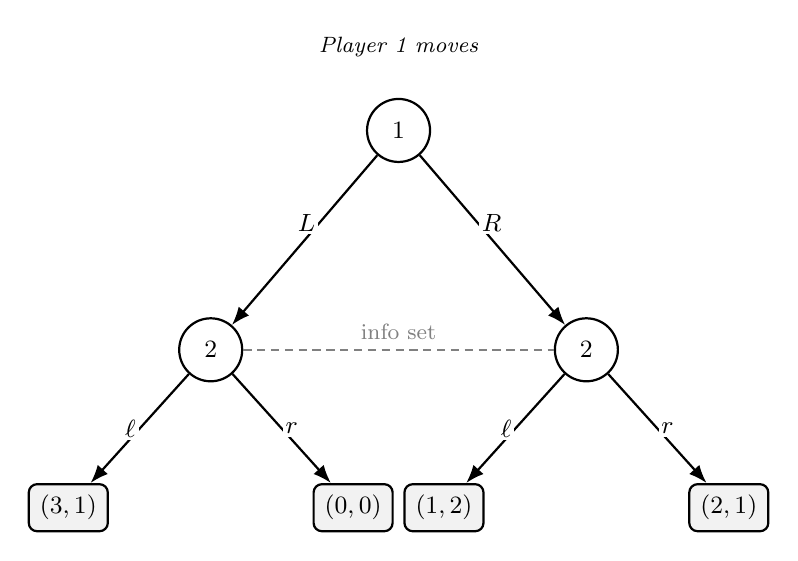
\begin{tikzpicture}[diagram base, node distance=22mm and 18mm]
% Root node (Player 1)
\node[player node] (r) {$1$};

% Player 2 decision nodes
\node[player node, below left=of r] (p2L) {$2$};
\node[player node, below right=of r] (p2R) {$2$};

% Terminal nodes with payoffs
\node[terminal node, below left=14mm and 10mm of p2L] (zLL) {$(3,1)$};
\node[terminal node, below right=14mm and 10mm of p2L] (zLR) {$(0,0)$};
\node[terminal node, below left=14mm and 10mm of p2R] (zRL) {$(1,2)$};
\node[terminal node, below right=14mm and 10mm of p2R] (zRR) {$(2,1)$};

% Edges from root
\draw[->, thick] (r) -- node[edge label, left, pos=0.4] {$L$} (p2L);
\draw[->, thick] (r) -- node[edge label, right, pos=0.4] {$R$} (p2R);

% Edges from Player 2 nodes
\draw[->, thick] (p2L) -- node[edge label, left] {$\ell$} (zLL);
\draw[->, thick] (p2L) -- node[edge label, right] {$r$} (zLR);
\draw[->, thick] (p2R) -- node[edge label, left] {$\ell$} (zRL);
\draw[->, thick] (p2R) -- node[edge label, right] {$r$} (zRR);

% Information set (curved line connecting P2 nodes)
\draw[info set] (p2L) -- node[above, font=\footnotesize, text=gray] {info set} (p2R);

% Player labels
\node[above=4mm of r, font=\footnotesize\itshape] {Player 1 moves};
\end{tikzpicture}
\caption{An extensive-form game tree. Player 1 chooses $L$ or $R$; then Player 2 moves without observing Player 1's choice. The dashed line connecting Player 2's nodes indicates an \emph{information set}: Player 2 cannot distinguish which node they are at.}
\label{fig:extensive-form}
\end{figure}

\paragraph{Minimax and the special structure of zero-sum games.}
Two-player zero-sum games have a very clean theory because the players’ objectives are exactly opposed. For a payoff matrix \(M\in \mathbb{R}^{m\times k}\) giving player 1’s payoff \(u_1(i,j)=M_{ij}\) (and player 2’s payoff \(-M_{ij}\)), mixed strategies \(x\in \Delta([m])\), \(y\in \Delta([k])\) yield value \(x^\top M y\). The central result is the minimax theorem:
\[
\max_{x\in \Delta([m])}\min_{y\in \Delta([k])} x^\top M y
=
\min_{y\in \Delta([k])}\max_{x\in \Delta([m])} x^\top M y
= v,
\]
and moreover there exist optimal mixed strategies \(x^\star,y^\star\) achieving the value \(v\). Conceptually, this says that in zero-sum games there is not much ambiguity about what "rational play" should mean: optimal play can be defined as a saddle point, and equilibrium is literally solving a convex-concave optimization problem. This theorem, and the broader mathematical framing of games as objects worth analyzing in their own right, is closely associated with von Neumann’s foundational work and his collaboration with Morgenstern. Good examples of two-player zero-sum games with perfect information are chess and Go.

\paragraph{Nash equilibrium in general-sum games.}
Zero-sum games are unusually clean because the players’ objectives are perfectly opposed, so there is a single "value" the game is trying to realize. General-sum games are subtler: there is no single scalar objective to optimize, and stability has to be defined in terms of deviations. A mixed-strategy profile \(\sigma^\star\) is a \emph{Nash equilibrium} if for every player \(i\),
\[
u_i(\sigma_i^\star,\sigma_{-i}^\star)\;\ge\;u_i(\sigma_i,\sigma_{-i}^\star)
\quad \forall\,\sigma_i\in \Delta(A_i).
\]
Equivalently, \(\sigma_i^\star\) is a best response to \(\sigma_{-i}^\star\) for each \(i\). Nash’s theorem shows that every finite normal-form game admits at least one mixed-strategy Nash equilibrium. For extensive-form games, one typically refines Nash to handle dynamic consistency and off-path behavior (subgame-perfect equilibrium or sequential equilibrium), but the key idea is the same: a stable profile is one where no player can profitably deviate given what the others are doing.

At this point, it is worth emphasizing one theme that will come back later. Game theory does not just give you a single prediction rule. It gives you a family of solution concepts, and which one you pick is part of your modeling assumptions.

Across these settings, game theory supplies a menu of equilibrium and solution concepts, only a few noted here. Some other well-known ones are Quantal Response Equilibrium, correlated equilibrium, coarse correlated equilibrium, Berge equilibrium, and many more. Each comes with different assumptions and different computational tradeoffs.

There are also other formalisms and granularities. Some are defined by structure (potential games), some by symmetry (symmetric versus asymmetric games), and some by how you access the game (explicit payoff tables versus simulator-based games where you cannot write down utilities in closed form). We also have not even touched on computational and algorithmic game theory, mechanism design (often dubbed reverse game theory), information design, fair division, social choice, voting, and connections to control theory and reinforcement learning. I am not going to try to cover everything here. The goal is just to set up the pieces we need so that when we bring in causality, the mapping is clear.

\subsection{Causality}
Causality is the mathematical and philosophical study of \emph{what changes when we change something}. Standard probabilistic modeling is usually about associations such as \(P(Y \mid X=x)\). Causal modeling aims to formalize \emph{interventions} (forcing \(X\) to take a value) and \emph{counterfactuals} (what would have happened under a different intervention, for the same underlying unit or world). This has led to formal frameworks, most notably Pearl's~\cite{pearl2009causality}, that specify (i) how the world generates data, (ii) what it means to intervene, and (iii) when such questions are identifiable from observations.

If game theory is about stability under deviations, causality is about stability under surgery. The whole point of this post is that, in traditional structural strategic settings, how do those two kinds of counterfactuals collide in interesting ways.

\paragraph{Structural causal models (SCMs).}
One clean formalism is a \emph{structural causal model}. An SCM is a tuple
\[
\mathcal{M} = (U, V, F, P(U)),
\]
where \(U\) are exogenous (background) variables, \(V=\{V_1,\dots,V_d\}\) are endogenous variables, \(F=\{f_1,\dots,f_d\}\) are structural assignments
\[
V_j = f_j(\mathrm{Pa}_j, U_j), \qquad j=1,\dots,d,
\]
and \(P(U)\) is a distribution over exogenous variables. The directed graph induced by these assignments (edges \(\mathrm{Pa}_j \to V_j\)) is the \emph{causal graph}. The key point is that \(F\) encodes how each variable is generated from its direct causes and noise, not just how variables are correlated.

% ----------------
% Diagram: an SCM
% ----------------

\begin{figure}[htbp]
\centering
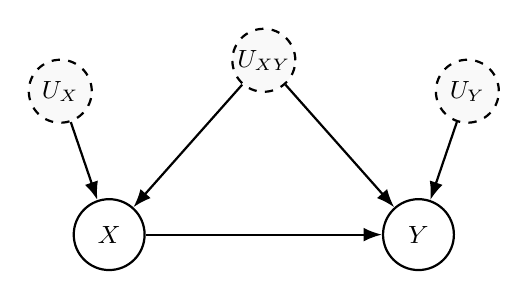
\begin{tikzpicture}[diagram base]
% Endogenous variables (main row)
\node[endo node] (X) {$X$};
\node[endo node, right=30mm of X] (Y) {$Y$};

% Exogenous variables (above, with clear layout)
\node[exo node, above left=12mm and 0mm of X] (Ux) {$U_X$};
\node[exo node, above right=12mm and 0mm of Y] (Uy) {$U_Y$};
\node[exo node, above=18mm of $(X)!0.5!(Y)$] (Uxy) {$U_{XY}$};

% Causal edges
\draw[->, thick] (X) -- (Y);

% Exogenous influences
\draw[->, thick] (Ux) -- (X);
\draw[->, thick] (Uy) -- (Y);
\draw[->, thick] (Uxy) -- (X);
\draw[->, thick] (Uxy) -- (Y);
\end{tikzpicture}
\caption{A structural causal model (SCM). Endogenous variables $X$ and $Y$ (solid nodes) are generated by structural assignments. Exogenous noise variables (dashed nodes) represent unobserved factors: $U_X$ and $U_Y$ are independent noise, while $U_{XY}$ is a common cause (confounder).}
\label{fig:scm}
\end{figure}

\paragraph{Interventions and the do-operator.}
An intervention \(\do(X=x)\) means we \emph{force} \(X\) to be \(x\) and break its usual generating mechanism. In an SCM, \(\do(X=x)\) is implemented by replacing the structural equation for \(X\) with the assignment \(X:=x\). The resulting interventional distribution is written \(P(Y \mid \do(X=x))\). This is not generally equal to \(P(Y \mid X=x)\), because the latter conditions on an event that may be confounded by common causes of \(X\) and \(Y\).

% -------------------------------
% Diagram: do-operator intuition
% -------------------------------
\begin{figure}[htbp]
\centering
\begin{subfigure}[b]{0.45\linewidth}
\centering
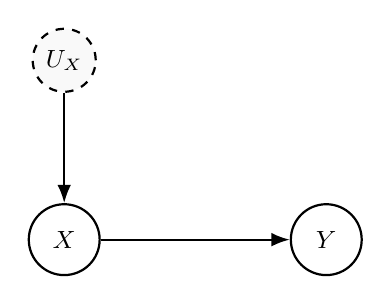
\begin{tikzpicture}[diagram base]
\node[exo node] (Ux) {$U_X$};
\node[endo node, below=14mm of Ux] (X) {$X$};
\node[endo node, right=24mm of X] (Y) {$Y$};
\draw[->, thick] (Ux) -- (X);
\draw[->, thick] (X) -- (Y);
\end{tikzpicture}
\caption{Observational regime}
\label{fig:do-obs}
\end{subfigure}
\hfill
\begin{subfigure}[b]{0.45\linewidth}
\centering
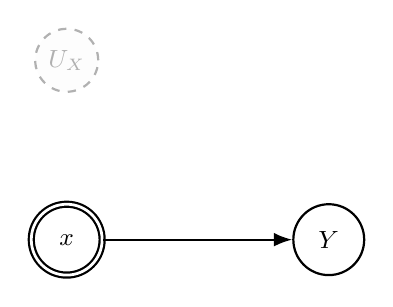
\begin{tikzpicture}[diagram base]
\node[exo node, opacity=0.3] (Ux) {$U_X$};
\node[endo node, below=14mm of Ux, double, double distance=1pt] (X) {$x$};
\node[endo node, right=24mm of X] (Y) {$Y$};
\draw[->, thick] (X) -- (Y);
\end{tikzpicture}
\caption{After intervention $\do(X{=}x)$}
\label{fig:do-int}
\end{subfigure}
\caption{The do-operator in action. (a) Under observation, $X$ is generated by its structural equation including noise $U_X$. (b) Under $\do(X{=}x)$, the mechanism is replaced: $X$ is fixed to value $x$, severing the edge from $U_X$.}
\label{fig:do-intervention}
\end{figure}

A central object is the \emph{average causal effect} (ACE), for instance,
\[
\mathrm{ACE} = \mathbb{E}[Y \mid \do(X=1)] - \mathbb{E}[Y \mid \do(X=0)],
\]
which extends naturally to continuous or multivalued treatments.

From this foundation, we can define Bayesian networks (BNs) and causal Bayesian networks (CBNs). A BN is a DAG \(G=(V,E)\) together with conditional probability distributions (CPDs) \(\{P(V_j \mid \mathrm{Pa}_j)\}_{j=1}^d\) such that the joint factorizes as
\[
P(v_1,\dots,v_d) =
\prod_{j=1}^d P\bigl(v_j \mid \mathrm{Pa}_j\bigr).
\]
This is purely probabilistic: it encodes conditional independences and provides an efficient representation for inference and likelihood-based modeling. A CBN is a BN whose edges are additionally interpreted as \emph{direct causal relationships}. The difference is semantic but important. In a CBN the graph is not just a compact factorization, it is also a claim about how the data is generated. This added semantics is exactly what allows interventions to be defined.

% ---------------------
% Diagram: a BN DAG
% ---------------------

\begin{figure}[htbp]
\centering
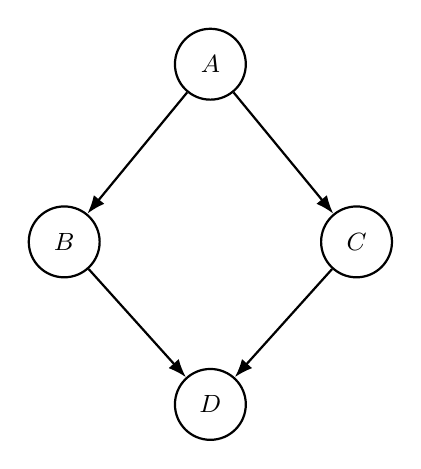
\begin{tikzpicture}[diagram base, node distance=18mm]
% Top node
\node[endo node] (A) {$A$};

% Middle layer
\node[endo node, below left=16mm and 12mm of A] (B) {$B$};
\node[endo node, below right=16mm and 12mm of A] (C) {$C$};

% Bottom node (centered between B and C)
\node[endo node, below=16mm of $(B)!0.5!(C)$] (D) {$D$};

% Edges
\draw[->, thick] (A) -- (B);
\draw[->, thick] (A) -- (C);
\draw[->, thick] (B) -- (D);
\draw[->, thick] (C) -- (D);
\end{tikzpicture}
\caption{A Bayesian network DAG encoding conditional independence structure. The joint distribution factorizes as $P(A,B,C,D)=P(A)\,P(B\mid A)\,P(C\mid A)\,P(D\mid B,C)$.}
\label{fig:bn}
\end{figure}

\paragraph{From SCMs to BNs.}
If an SCM \(\mathcal{M}=(U,V,F,P(U))\) is acyclic, then it induces a BN over \(V\) by pushing forward \(P(U)\) through the structural equations. Under standard conditions (for example independent exogenous noises), the induced distribution over \(V\) factorizes according to the causal graph:
\[
P(v) =
\prod_{j=1}^d P\bigl(v_j \mid \mathrm{Pa}_j\bigr).
\]
So: SCM implies a causal DAG, which implies a BN factorization for \(P(V)\). But the converse is not true without extra assumptions: many different SCMs can induce the same observational BN and CBN. The usefulness of causal graphs is that interventions on them have clear and useful meanings.

\section{Work to bridge ideas from the two}
\subsection{Bridging the two: MAIDs and causal games}
One classic structural connection between causality and game theory is the \emph{Multiagent Influence Diagram} (MAID), introduced by Koller and Milch~\cite{koller2003maid}. The framework presented in this section draws heavily on the work of Hammond et al.~\cite{hammond2023causality}, which extends MAIDs to full \emph{causal games}.

A MAID is a structure $\mathcal{M} = (\mathcal{G}, \boldsymbol{\theta})$ where $\mathcal{G} = (N, \mathbf{V}, E)$ specifies a set of agents $N=\{1,\dots,n\}$ and a DAG $(\mathbf{V}, E)$. The node set $\mathbf{V}$ is partitioned into chance variables $\mathbf{X}$, decision variables $\mathbf{D}=\bigcup_{i\in N}\mathbf{D}^i$, and utility variables $\mathbf{U}=\bigcup_{i\in N}\mathbf{U}^i$. Parameters $\boldsymbol{\theta}=\{\theta_V\}_{V\in\mathbf{V}\setminus \mathbf{D}}$ define conditional probability tables for each non-decision variable, so that (once decisions are specified) the model induces a Bayesian network over the chance and utility nodes.

Here is the intuition that I like to keep in mind. A MAID is a probabilistic graphical model, but it is wired up so that some nodes are controlled by strategic agents. So it is already halfway between a causal graph and a game tree.


\begin{figure}[htbp]
\centering
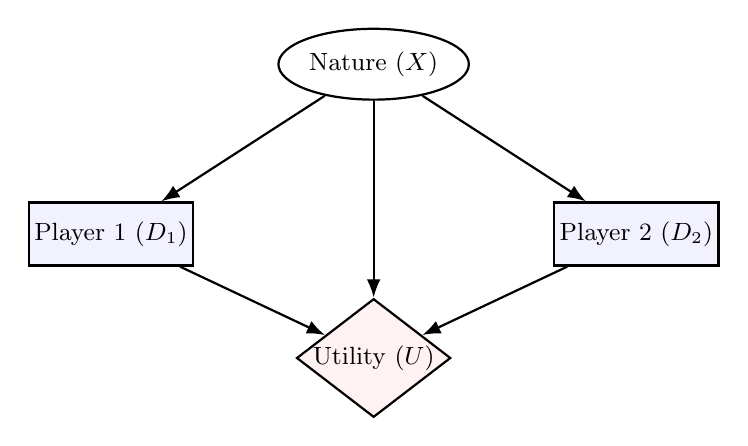
\begin{tikzpicture}[diagram base, node distance=20mm]
  \node[maid chance] (X) {Nature ($X$)};
  \node[maid decision, below left=of X] (D1) {Player 1 ($D_1$)};
  \node[maid decision, below right=of X] (D2) {Player 2 ($D_2$)};
  \node[maid utility, below=25mm of X] (U) {Utility ($U$)};
  \draw[->, thick] (X) -- (D1); 
  \draw[->, thick] (X) -- (D2); 
  \draw[->, thick] (D1) -- (U);
  \draw[->, thick] (D2) -- (U);
  \draw[->, thick] (X) -- (U);
\end{tikzpicture}
\caption{A MAID following standard conventions: Decisions (Rectangles), Utilities (Diamonds), and Chance (Ovals).}
\label{fig:maid-example}
\end{figure}

A key point is that in a MAID, \emph{strategies} become \emph{policies}: each agent $i$ chooses a collection of decision rules, one per decision node $D\in \mathbf{D}^i$, mapping the node's informational parents (denoted $\mathrm{Pa}_D$) into an action distribution. Writing the full policy profile as $\pi=(\pi^1,\dots,\pi^n)$, the MAID together with $\pi$ induces a well-defined joint distribution $P^\pi$ over all variables, hence well-defined expected utilities.

From here we can define a Nash equilibrium directly at the level of policies. A policy profile $\pi^\star$ is a \emph{Nash equilibrium} in a MAID $\mathcal{M}$ if for every agent $i\in N$,
\[
\pi^{i,\star} \in \argmax_{\hat{\pi}^i \in \Pi^i}
\;\;\sum_{U\in\mathbf{U}^i}\; \mathbb{E}_{P^{(\hat{\pi}^i,\pi^{-i,\star})}}[U],
\]
where $\Pi^i$ is the set of valid policies for agent $i$, and $P^{(\hat{\pi}^i,\pi^{-i,\star})}$ is the distribution induced when agent $i$ deviates to $\hat{\pi}^i$ while others play $\pi^{-i,\star}$. This mirrors the usual deviation-based definition in normal-form and extensive-form games, but now the probability model is built into the graph.

\paragraph{Mechanised MAIDs and making causality explicit.}
A MAID already looks like a causal graph, but there is a subtlety: the distribution $P^\pi$ depends on the agents' policies, yet policies are not random variables. They are chosen strategically. A \emph{mechanised MAID} makes this dependence explicit by augmenting the graph with additional structure: for each decision node $D$, we introduce a \emph{policy node} $\Pi_D$ that parameterizes the decision rule, along with edges from information parents to the policy node and from the policy node to $D$. This lets us distinguish two types of interventions:
\begin{enumerate}
  \item[(i)] \textbf{Interventions on the environment}: modifying chance nodes or the information structure (which edges exist);
  \item[(ii)] \textbf{Interventions on policies}: directly setting $\do(\Pi_D = \pi_D)$ to fix a decision rule.
\end{enumerate}
This is the key move that makes causal language feel natural. Once policies are explicit objects in the model, you can talk about intervening on them, not just conditioning on them.

\subsection{Making use of these structures: what does it mean to ask a causal question in a game?}
Once you see the MAID as a probability model \emph{conditional on a policy profile}, you can start asking causal questions. But you quickly run into a very game-theoretic issue: the model does not pick a single distribution for you. In a standard causal model, there is one data generating process. In a game, there is often a \emph{set} of plausible data generating processes, because there may be multiple "rational" policy profiles (multiple equilibria, or multiple outcomes under whatever refinement you believe in).

\paragraph{Queries are often set-valued.}
Let $\mathsf{Sol}(\mathcal{M})$ denote the set of "rational" policy profiles for the MAID under a chosen solution concept. Then a prediction query like
\[
P(Y \mid X=x)
\]
is not a single number anymore, but a family of answers indexed by $\pi\in\mathsf{Sol}(\mathcal{M})$. In other words, the natural output is the \emph{set}
\[
\Big\{\, P^{\pi}(Y \mid X=x) : \pi\in\mathsf{Sol}(\mathcal{M}) \,\Big\},
\]
where $P^{\pi}(\cdot)$ is the distribution induced by the MAID when agents play policy profile $\pi$. This sounds annoying at first, but it is actually honest. Without an equilibrium selection story, the game itself does not identify a unique forecast.

If you want a single prediction, you can always add an equilibrium selection rule. But it is helpful to notice when that selection rule is doing work, because it changes what you mean by "the" outcome of the game.

\paragraph{Pre-policy vs.\ post-policy interventions.}
In Pearl-style causality, an intervention $\do(Z=z)$ replaces the mechanism generating $Z$. In a strategic setting, we also have to say whether agents get to respond to the intervention, or whether their decision rules are treated as fixed.

Hammond et al.~\cite{hammond2023causality} formalize this distinction in a way that I find really useful. There are two different meanings that both deserve to be called "causal":

\begin{itemize}
  \item \textbf{Post-policy intervention (hold decision rules fixed).} Fix a policy profile $\pi$ (for example a particular equilibrium, or any other policy profile of interest), and then apply an intervention to the non-decision part of the model while \emph{keeping the policies fixed}. This produces an interventional distribution of the form
  \[
  P^{\pi}(Y \mid \do(Z=z)).
  \]
  Intuitively, this isolates a direct causal effect within a fixed behavior model: what changes if we surgically modify part of the environment or information structure, without allowing strategic re-optimization.

  \item \textbf{Pre-policy intervention (allow strategic response).} Apply the intervention first, producing a modified MAID $\mathcal{M}_{\do(Z=z)}$, and then consider rational play in the intervened game. The natural output is again set-valued:
  \[
  \Big\{\, P^{\pi'}(Y) : \pi' \in \mathsf{Sol}(\mathcal{M}_{\do(Z=z)}) \,\Big\}.
  \]
  Intuitively, this captures strategic adaptation: you changed the rules of the world, so the set of rational policies may change.
\end{itemize}

The important point is that these answer different questions. Post-policy isolates a direct causal effect holding behavior fixed, while pre-policy includes the downstream effect of equilibrium adjustment. If you are not explicit about which one you mean, you can end up talking past people, because the two effects can differ a lot.

\paragraph{Counterfactuals require more structure.}
There is a second subtlety: for \emph{counterfactuals} you typically want a structural model, not just a Bayesian network. A counterfactual wants to reuse the same background noise $U$ across the factual and counterfactual worlds (same underlying world, different intervention). So to talk about "what would have happened in the same world if we had changed $Z$" you want structural equations for the chance variables. When you add that structure to the game, you can ask counterfactual questions, again typically indexed by which rational outcome you assume.

\paragraph{Relation to extensive-form games.}
At this point it is natural to ask, why not just use extensive-form games (EFGs) and do everything there? The short answer is that MAIDs and EFGs are two views of the same underlying object. You can unroll a MAID into an extensive-form representation (often with blowup), and you can sometimes compress an extensive-form game into a MAID by exploiting conditional independence and repeated structure. The payoff is that MAIDs are closer in spirit to causal graphs, so causal questions about information flow and interventions are easier to express without drowning in the tree.

\paragraph{Other Perspectives}
Another direction I like at this intersection flips the problem around. Instead of asking how to make games causal, it asks what happens to causal inference when agents are strategic. In many real settings, treatments are not purely exogenous assignments. There can be competition over who gets treated, incentives to manipulate assignment, and strategic responses to being experimented on. Once you take that seriously, equilibrium concepts start showing up even if your end goal is statistical estimation, because the data you observe may itself be a strategic outcome of an incentive system. This suggests a deep link between mechanism design, game theory and strategic interference in control trials: questions I will begin to explore in a later post.

\begin{thebibliography}{9}

\bibitem{hammond2023causality}
Lewis Hammond, James Fox, Tom Everitt, Ryan Carey, Alessandro Abate, and Michael Wooldridge.
\newblock Reasoning about causality in games.
\newblock \emph{Artificial Intelligence}, 320:103919, 2023.

\bibitem{koller2003maid}
Daphne Koller and Brian Milch.
\newblock Multi-agent influence diagrams for representing and solving games.
\newblock \emph{Games and Economic Behavior}, 45(1):181-221, 2003.

\bibitem{pearl2009causality}
Judea Pearl.
\newblock \emph{Causality: Models, Reasoning, and Inference}.
\newblock Cambridge University Press, 2nd edition, 2009.

\end{thebibliography}

\end{document}